\chapter{Prediction with Commit Data}
\label{chap:prediction}

% TODO discuss research question **************************************************************************************************

% How the visualization helped 	
The visualization for the data collected from the projects helps provide several insights into data set which can be used to help with the creation of the prediction scheme. With the data visualized, a more general look of the data collected is available. While creating the method for predicting change within the project, the visualizations provide a helpful resource. The visualization can help identify relationships between variables and general trends. The actual data used for training the prediction model is outlined in \autoref{sec:prediction_data}. After that the prediction model is detailed in \autoref{sec:prediction_method}. %Finally, the actual implementation is discussed in \autoref{sec:implementation}

The data presented in the visualization is used towards creating an approach to predict whether a method will change within the next five commits. The machine learning algorithms used in the approach are \gls{svm} and \gls{rf}. Of course the performance of a prediction method will be influenced by several factors including; the size of the sample, the features used for training and balancing of the data set.

\section{Prediction Data}
\label{sec:prediction_data}

The data used to predict changes within a project is originally from the visualizations. For more information about the specific information collected see: \autoref{sec:collection}, \autoref{sec:storage} and \autoref{sec:parsing}. The commit data collected from the target \gls{oss} project is used to make predictions. The goal is to predict whether a method within a project will change within the next five commits. As outlined in \autoref{sec:parsing}, the different types of changes can be either additions, deletions, modifications or no change at all.

The machine learning model requires samples from the data set to train from which allows for predictions of new elements. The training samples taken must also be categorized based on the desired outcome of the machine learning algorithm. This requirement provides some restrictions on which values can be included in the sampling. Since the categorization is whether a method will change, all methods sampled need to be able to collect data the next five commits following the current commit. Therefore methods that are within the last five commits of the training sample window are not included in the training set for the data model.

\begin{figure}[!ht]
    \centering
        %Generated from http://jsfiddle.net/u43dfLxp/1/
        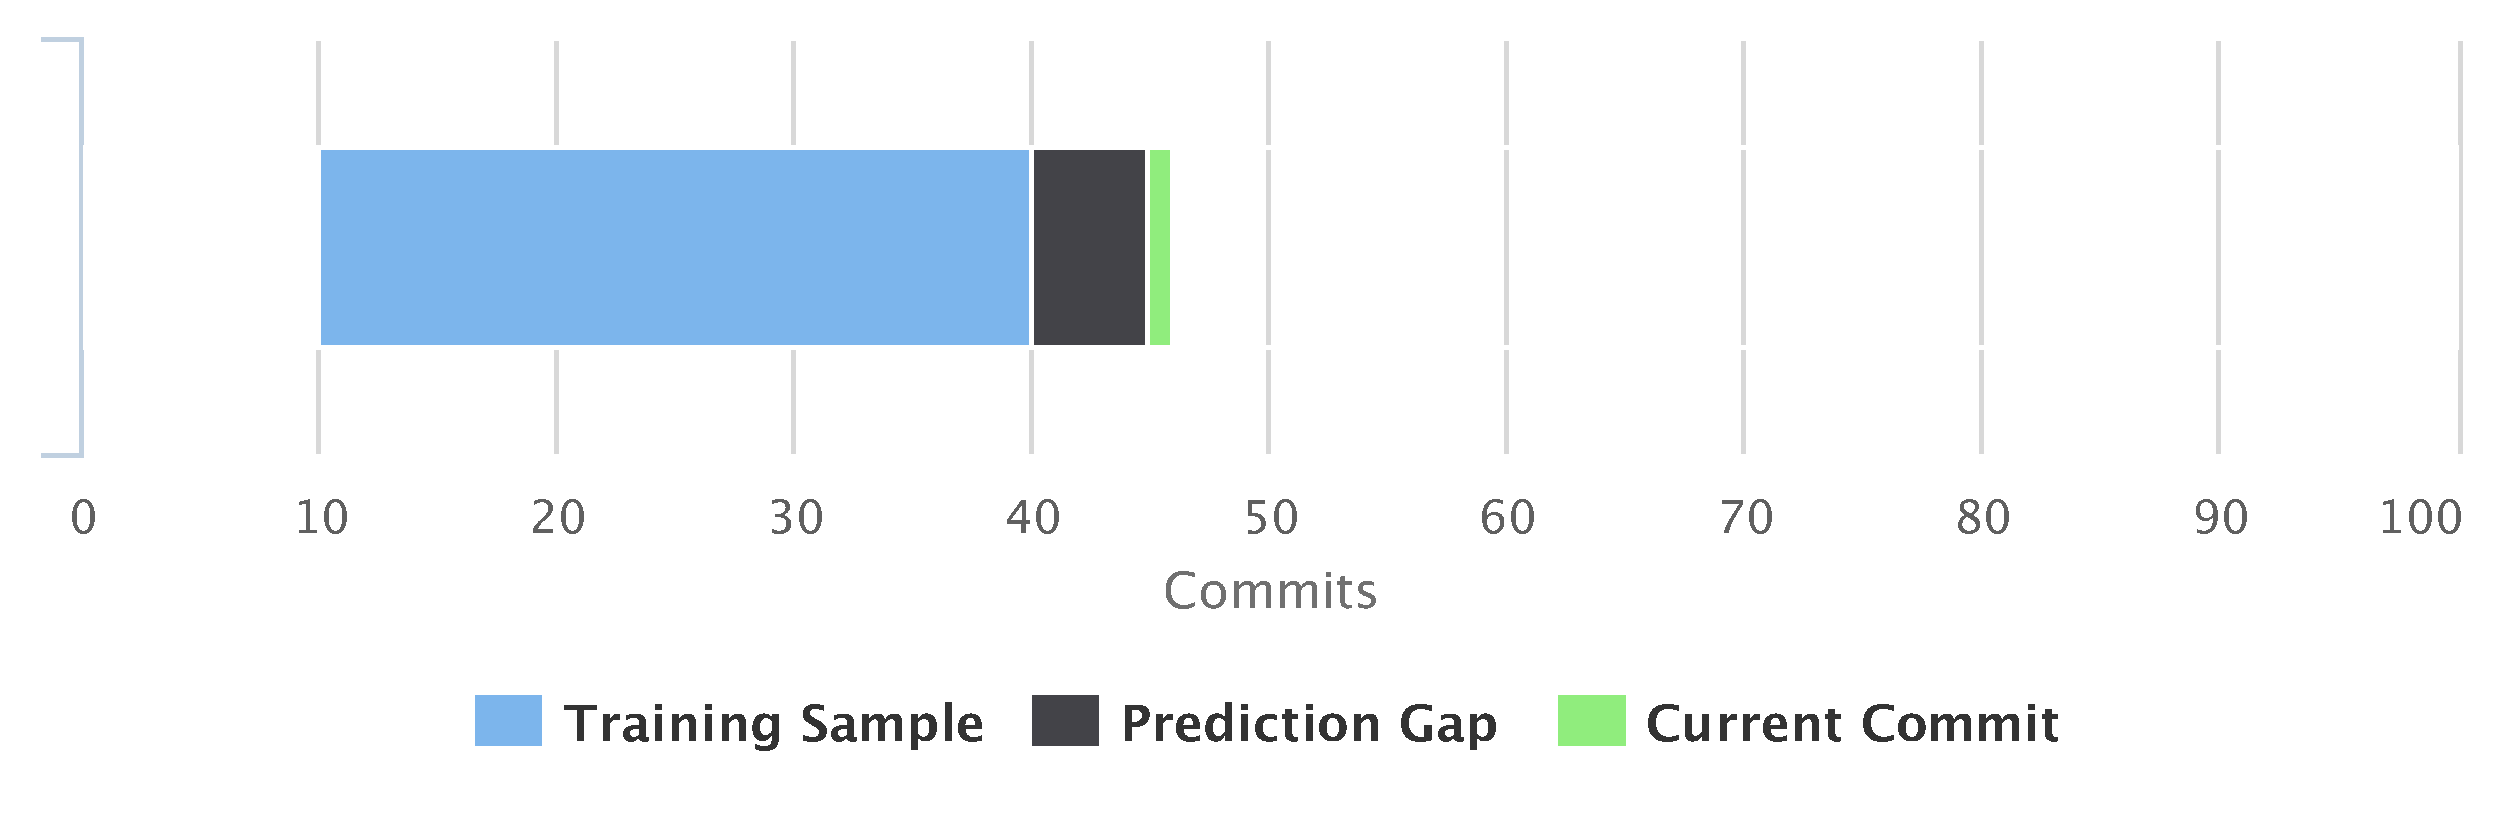
\includegraphics[width=1.0\textwidth]{images/training_sampling}
    \caption{Training Sampling Layout}
    \label{fig:training_data_range}
\end{figure}

As noted above, one of the key factors in the performance of the prediction approach is the size of the sample set. The sample set size is restricted by a variable value \gls{swr} which controls the number of commits considered to sample from. The data will only be sampled within a limited range of commits as outlined in \autoref{fig:training_data_range}. In this case, the \gls{swr} is 30 and the prediction gap is 5. The prediction gap takes into account the categorization restriction, preventing sampling from the last five commits.

Another consideration when sampling the data is the distribution of the categories. Most of the time, a data set will contain more samples in one category than the other. For example, a sample may contain $80\%$ methods with no change within the next five commits and $20\%$ methods with change. Ideally the number of methods with changes and without changes in the next five commits would be close to $50\%$. When the distribution of samples for each category is very close the model will often perform better. However in cases where the data is highly skewed to one classification over the other, the model will often predict the larger classification for input values. \gls{os} will re-samples from the smaller classification to reduce the size difference with the larger classification. Alternatively, undersampling the data set will remove samples from the larger classification to reduce the difference in size with the smaller classification.

% Discussed further in section in approach
Undersampling is applied to a data set by measuring the number of samples in each category. The larger of the two is reduced by discarding samples at random until the data set is the same size as the smaller data set. This will reduce the number of samples used to train the model and may reduce the performance of the model based on the decreased number of samples. In cases where there are a limited number of samples for the smaller category, undersampling may not be ideal. \gls{os} alternatively increases the number of samples by calculating the number of samples in each category and expanding the smaller category by re-sampling values from the data set until both categories are equal in size. Both approaches can be used together so that the smaller category is expanded to at most twice its original size. If the initially smaller category is still smaller, the larger category set will be reduced to the size of the smaller category. When selecting values for re-sampling or removal, a randomized selection process is used to ensure the distribution of the data is preserved. For example, if category $a$, with $|a| = 100$ and category $b$ with $|b| = 1000$. \gls{os} will be applied to category $a$ since $|a| < |b|$. Therefore $a$ will apply random re-sampled until $|a_n| = |a| \times 2$ or $|a_n| = |b|$. Once one of the conditions is met, \gls{os} is complete. Next undersampling is applied to the larger category $b$, where samples are randomly removed from $b$ until $|b_n| = |a_n|$.

% Discuss the percentage of sampling.
Once the categories are balanced then the model can use the data. However with large sample sizes, a reduction of the sample set may be necessary. The variable $sample_r$ is the percentage of the number of samples taken from the range. Instead of picking an arbitrary number of samples, a ratio was used to scale based on the number of available samples. When sampling, if the ratio is at $50\%$ then only half of the values retrieved will be used to train or test. For some of the larger data sets sampling $100\%$ of the data from the range would take a lot longer. Therefore sampling a percentage of the data set is commonly used to decrease the training time. In order to provide a more stable model, a random sample of the sample range is used so that each data entry in the sample has the same chance to be within the training or test data set. Using the example from above, $a$ and $b$ have been oversampled and undersampled such that their new sizes are represented by $|a_n|$ and $|b_n|$ respectively. Given that a sample ratio of $50\%$ is used then both sets $a$ and $b$ would be reduced by the ratio by randomly sampling from each set to create new sets. The size of each set would be $|a_n| \times r$ where $r$ is the ratio value.

% TODO outline initial set of features used
% List of features that were used initially:
% - change type, the type of change the method received (eg. 0-> no change, 1-> newly addded, 2 -> deleted, 3 -> modified)
% - changed, whether the method changed or not (e.g 0-> no change, 1 -> changed)
% - prev change type_i, the change type for n-i commit of the method
% - changed_i, whether a change occured for n-i commit of the method
% - previous time interval, the difference in commit times for the method changes i and j.
%
% - percentage of method change (sum(lines changed)/ sum(lines unchanged))

%238, ReportField.java            |           8234 | public boolean getValue() {                                                                          |           0 | william-ferguson-au |  0.0464135021097046 | ("{3,3,0,0,0}","{68,1816,549469,779372,208198}")                              |        0
\begin{table}
\begin{center}
    \begin{tabularx}{\linewidth}{|l|X|l|l|}
        \hline
        Feature & Description & Data & Example \\
         & & & Vector \\
        \hline
        Com & The individual who committed the change & bob & 5 \\ \hline
        Sig & The method signature related to the change details & void getValue() & 46\\ \hline
        Name & The name of the file & Main.java & 3 \\ \hline
        $\Delta_i$ & Whether the method changed or not in the current commit & 3 & 1 \\ \hline 

        %$type_{\Delta}$ & Type of change made to the method & 3 & 3 \\ \hline
        $m_+$ & Whether the is newly added & 3 & 0 \\ \hline
        $m_-$ & Whether the method was deleted & 3 & 0 \\ \hline
        $m_c$ & Whether the is a modification & 3 & 1 \\ \hline
        $m_x$ & Whether the received no change & 3 & 0 \\ \hline

        $\Delta_{i-j}$ & Whether the method changed in a previous commit & 0 & 0 \\ \hline

        $type_{\Delta_{i-j}}$ & Type of method changed in a previous commit & 2 & 2 \\ \hline
        
        $f_{\Delta}$ & The frequency that the method is changed within the \gls{swr} & 0.0464 & 0.0464 \\ \hline
        $sf_{\Delta}$ & The frequency that the method is changed within the last 10 commits.  & 0.1 & 0.1 \\ \hline
        $t_\Delta$ & The time between the current commit $c_i$ and the previous commit $c_{i-1}$ & 2148 & 2148 \\ \hline

        $t_{\Delta_{i-j}}$ & The time difference between a sequence of two previous commits & 453 & 453 \\ \hline

        Length & The length of the method in this commit & 10 & 10 \\ \hline
        $change_{t-1}$ & Whether a change has occurred in the previous 5 commits & $\{3, 0, 0, 3, 0\}$ & 1 \\
        \hline
        $change_{t}$ & Identifies whether a change occurred within the next 5 commits for the given method & 0 & 0\\
        \hline
    \end{tabularx}
\end{center}
    \caption{Candidate features for \gls{svm} model}
    \label{tab:candidate_features}
\end{table}

% Name => Methods within a file are likely going to have similar change patterns
% Signature => A method change history will likely be unique
% Change_i => Whether the method changed or not at the current commit may provide insight as to whether the next 5 commits will feature a change as well.
% committer => Users may change in different change patterns thus helping identify whether this will be a change or not, 
% freq_change => Helps identify how likely the file is to change

The \autoref{tab:candidate_features} outlines each of the considered features used for training the prediction model. An example of each feature is provided to further illustrate the feature. As stated in the previous \autoref{subsec:svm_prediction}, the values need to be processed into a usable format for \gls{svm} or \gls{rf}. First the data is extracted from the database as \textit{raw} values as shown in the \textit{\textbf{Data}} column. Text values are mapped to a integer value. For example the \textit{Name} value, ``Main.java'' will be mapped to the value 3. The reason the value is 3 is because 2 other methods have already been mapped and therefore method name is mapped to the next available mapping. Similarly both \textit{Com} and \textit{Sig} will be mapped from their respective values ``void getValue()'' and ``bob'' to 46 and 5. Numerical values are converted by casting the value to a floating point value if the value is not that type already. For spacing reasons, all the values in the table that have no decimal value are shown without a ``.0'' following.
%converted into floating point numbers.

Several experiments were conducted to investigate the value of each of the candidate features. The candidate features were narrowed down from this initial list into a smaller set of training features. These features sets were constructed to determine potential ideal feature sets. The complete list of features used are shown in \autoref{tab:training_features}. Some of the feature sets are not full explained in the table for spacing reasons. Feature sets 16, 17, 18 and 27 all use the last five previous changes or durations. Each are marked similarly to those that only use the most recent previous change or duration except for a footnote marker. Likewise feature set 29 is also different since the previous change used is only the change made five commits ago. Each of these feature sets are tested on the repository acra and the results are shown in \autoref{fig:feature_set_acra_rf}. 

\begin{figure}[!t]
    \centering
        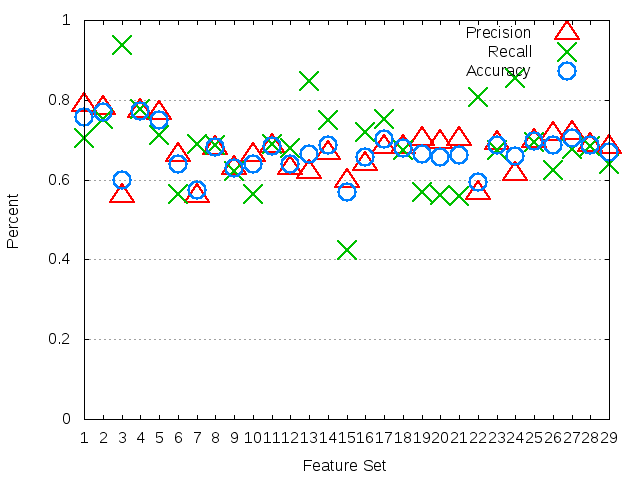
\includegraphics[width=0.8\textwidth]{images/rf/test_6/acra_sample_range}
        \caption{Feature Sets Analysis using \gls{rf}}
        \label{fig:feature_set_acra_rf}
\end{figure}



\begin{landscape}
\newgeometry{right=-3.1cm,bottom=15cm,footskip=10pt}
\thispagestyle{empty}
\begin{table}
\begin{center}
    \begin{tabular}{|c|c|c|c|c|c|c|c|c|c|c|c|c|c|c|c|c|}
        \hline
        Feature & Com & Sig & Name & $\Delta_i$ & $m_+$ & $m_-$ & $m_c$ & $m_x$ & $\Delta_{i-j}$ & $type_{\Delta_{i-j}}$ & $f_{\Delta}$ & $sf_{\Delta}$ & $t_\Delta$ & $t_{\Delta_{i-j}}$ & Length & $change_{t-1}$ \\
        Sets & & & & & & & & & & & & & & & & \\ 
        \hline
        1 & $\bullet$ & $\bullet$ & $\bullet$ & & & & & & & & $\bullet$ & $\bullet$ & & & $\bullet$ & $\bullet$ \\
        2 & $\bullet$ & $\bullet$ & $\bullet$ & & & & & & & & $\bullet$ & & $\bullet$ & & $\bullet$ & $\bullet$ \\
        3 & $\bullet$ & $\bullet$ & $\bullet$ & & & & & & & & $\bullet$ & & $\bullet$ & & & $\bullet$ \\
        4 & & $\bullet$ & $\bullet$ & & & & & & & & $\bullet$ & & $\bullet$ & & & $\bullet$ \\
        5 & $\bullet$ & $\bullet$ & $\bullet$ & & & & & & & & $\bullet$ & & & & & $\bullet$ \\
        6 & $\bullet$ & $\bullet$ & $\bullet$ & $\bullet$ & & & & & & & $\bullet$ & & & & & $\bullet$ \\
        7 & $\bullet$ & $\bullet$ & $\bullet$ & & $\bullet$ & & & & & & $\bullet$ & & & & & $\bullet$ \\
        8 & $\bullet$ & $\bullet$ & $\bullet$ & & & $\bullet$ & & & & & $\bullet$ & & & & & $\bullet$ \\
        9 & $\bullet$ & $\bullet$ & $\bullet$ & & & & $\bullet$ & & & & $\bullet$ & & & & & $\bullet$ \\
        10 & $\bullet$ & $\bullet$ & $\bullet$ & & & & & $\bullet$ & & & $\bullet$ & & & & & $\bullet$ \\
        11 & $\bullet$ & $\bullet$ & $\bullet$ & & & & & & $\bullet$ & & $\bullet$ & & $\bullet$ & & & $\bullet$ \\
        12 & $\bullet$ & $\bullet$ & $\bullet$ & & & & & & & $\bullet$ & $\bullet$ & & $\bullet$ & & & $\bullet$ \\
        13 & $\bullet$ & $\bullet$ & $\bullet$ & & & & & & & $\bullet$ & $\bullet$ & & & & & $\bullet$ \\
        14 & $\bullet$ & $\bullet$ & $\bullet$ & & & & & & $\bullet$ & & $\bullet$ & & & & & $\bullet$ \\
        15 & $\bullet$ & $\bullet$ & $\bullet$ & & & & & & & & $\bullet$ & & & $\bullet$ & & $\bullet$ \\
        16 & $\bullet$ & $\bullet$ & $\bullet$ & & & & & & $\bullet$ & & $\bullet$ & & & & & $\bullet$ \\ % Note this uses previous 5
        17 & $\bullet$ & $\bullet$ & $\bullet$ & & & & & & & $\bullet$ & $\bullet$ & & & & & $\bullet$ \\ % Note this uses previous 5
        18 & $\bullet$ & $\bullet$ & $\bullet$ & & & & & & & $\bullet$ & $\bullet$ & & $\bullet$ & & & $\bullet$ \\ % Note this uses previous 5
        19 & $\bullet$ & $\bullet$ & $\bullet$ & & $\bullet$ & $\bullet$ & $\bullet$ & & & & $\bullet$ & & & & & $\bullet$ \\
        20 & $\bullet$ & $\bullet$ & $\bullet$ & & & $\bullet$ & $\bullet$ & & & & $\bullet$ & & & & & $\bullet$ \\
        21 & $\bullet$ & $\bullet$ & $\bullet$ & & & $\bullet$ & & $\bullet$ & & & $\bullet$ & & & & & $\bullet$ \\
        22 & & $\bullet$ & $\bullet$ & & & & & & & & $\bullet$ & & & & & $\bullet$ \\
        23 & & $\bullet$ & $\bullet$ & & & & & & & & $\bullet$ & & & & & \\
        24 & & $\bullet$ & $\bullet$ & & & & & & $\bullet$ & & $\bullet$ & & & & & \\
        25 & & $\bullet$ & $\bullet$ & $\bullet$ & & & & & & & $\bullet$ & & & & & \\
        26 & & $\bullet$ & $\bullet$ & $\bullet$ & & & & & & & $\bullet$ & & $\bullet$ & & & \\
        27 & & $\bullet$ & $\bullet$ & $\bullet$ & & & & & $\bullet$ & & $\bullet$ & & & & & \\ % Note this includes 5 previous changes
        28 & & $\bullet$ & $\bullet$ & $\bullet$ & & & & & $\bullet$ & & $\bullet$ & & & & & \\
        29 & & $\bullet$ & $\bullet$ & $\bullet$ & & & & & $\bullet$ & & $\bullet$ & & & & & \\ % Uses change type from 5 previous commit (c_{i - 5})
        \hline
    \end{tabular}
    \caption{Training Features}
    \label{tab:training_features}
\end{center}
\end{table}
\restoregeometry
\end{landscape}
\thispagestyle{plain}




Another small change made to the data to create a vector for the prediction model was to convert the change type into a change indicator vector using \autoref{eq:change_type}. The vector is converted into a single value which indicates whether a change has occurred in the previous five commits. This process is done through calculating the sum of the change vector using \autoref{eq:change_reduce}. Finally, the change indicator, $change{i-1}$, is identified using \autoref{eq:change_prev}.

\begin{equation} 
\label{eq:change_type}
C = \left\{\begin{matrix}
1 & \text{if} change > 0 \\
0 & \text{otherwise}
\end{matrix}\right.
\end{equation}

\begin{equation} 
\label{eq:change_reduce}
reduce = \sum_{i=t-5}^{t}{c_i}
\end{equation}

\begin{equation} 
\label{eq:change_prev}
P = \left\{\begin{matrix}
1 & \text{if} reduce > 0 \\
0 & \text{otherwise}
\end{matrix}\right.
\end{equation}

$f_{\Delta}$ is calculated by taking the number commits in which involve changes to the current method ($c_i$) within the \gls{swr} divided by the current number of commits ($c_{cur}$) since the start of the \gls{swr}. This is formalized in \autoref{eq:freq_change}. A frequency of change is available for the duration of the \gls{swr}.

\begin{equation}
\label{eq:freq_change}
f_{\Delta} = \frac{|c_i|}{|c_{cur}|}
\end{equation}

$sf_{\Delta}$ is calculated by reducing the range sampled to $s$. Then counting the number of times the method changes within the last $s$ commits and dividing it by $s$. The size of the short frequency can be any value that is less than the size of the \gls{swr}. For use in the rest of the paper $s = 10$ which means that the $sf_{\Delta}$ is for the last $10$ commits.

%Both $change_{prev}$ and $\Delta t$ are actually each 5 features since they are a set of features. $change_{prev}$ shows the type of change that occurred for the last 5 commits. Similarly 

$t_\Delta$ is the difference between the current commit time ($t(c_i)$) and the previous commit time ($t(c_{i-1})$) calculated in \autoref{eq:time_delta}. Both time values are provided as time stamps and the result is calculated in seconds. Only the difference in time between the current commit and the previous one is calculated therefore, in \autoref{eq:time_delta}, $i$ denotes the current commit.

\begin{equation}
\label{eq:time_delta}
\Delta t_{i} = t(c_i) - t(c_{i-1}), i > 1
\end{equation}

\section{Prediction Method}
\label{sec:prediction_method}

% TODO talk about the machine learning algorithms more specifically:
% - Which are we using
% - Why did we choose them
% - what parameters they use
	% - What we set those parameters to
	% - and why

For this approach a machine learning algorithm is used to create a prediction model. The data used to train the model is collected as shown in \autoref{sec:prediction_data}. The machine learning algorithms that can be used are either \gls{svm} or \gls{rf}. Each of these method are widely used for data mining techniques and are easy to use. \autoref{fig:overview} outlines the overall structure of the approach for how changes are predicted.

% TODO either reference the overall architecture or create a more detailed version to show.

% TODO talk about how to set up the predictions for use (actual implementation)
	% - including what to expect from the approach and so on.
The \gls{svm} model was created through the use of a libsvm\footnote{\url{https://www.csie.ntu.edu.tw/~cjlin/libsvm/}} binding for Ruby, rb-libsvm\footnote{\url{https://github.com/febeling/rb-libsvm}}. This library was a good fit since the data was collected using a Ruby script. For \gls{rf} python library scikit-learn\footnote{\url{http://scikit-learn.org/stable/}} was used. The reason for switching from Ruby to Python was a lack of a mature library for \gls{rf} in Ruby.

Use of the approach requires a few steps in total before predictions can begin. Firstly, the data related to the project must be collected from GitHub. Once the data is collected, the prediction model can be created by providing training set built from sampling the data set. After training the model, predictions can be made using the model on new data. The next chapter analysis the approach by training and testing the model using subsets of the project data sets.